% book/index.tex —— 封面、目录与全书章节索引（对应模板的 book/index.tex）
% 想调整章节顺序：直接移动下面的行即可

\begin{center}
\thispagestyle{empty}
\begin{tikzpicture}[remember picture, overlay, inner sep=0pt]
\node at (current page.center)
{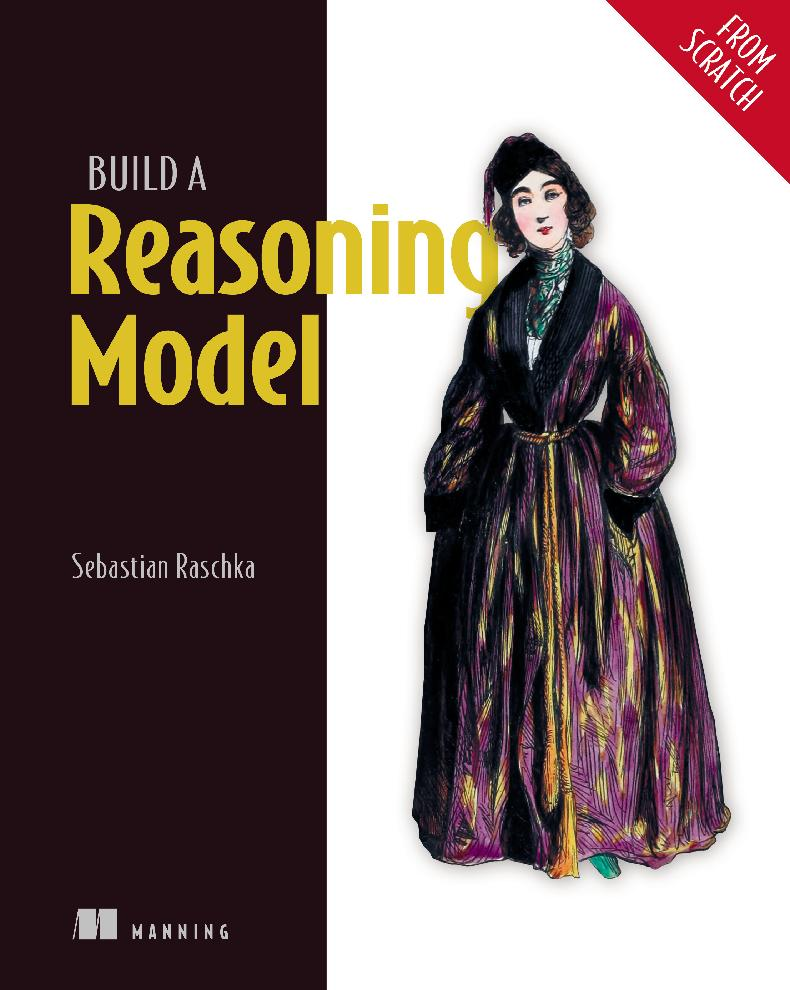
\includegraphics[width=\paperwidth, keepaspectratio=false]{images/cover.jpg}};
\end{tikzpicture}
\newpage
\myGraphic{0.2}{images/manning_m.jpg}{}
\thispagestyle{empty}
\Huge
\textbf{从零构建推理模型}
\\[14pt]
\large
Build a Reasoning Model (From Scratch)
\\[14pt]
\normalsize
作者：Sebastian Raschka

如需评论，请访问 \href{https://livebook.manning.com/forum?product=raschka2}{livebook}。

\myGraphic{0.07}{images/Manning_M_small.png}{}

Manning Shelter Island

如需了解本书及更多 Manning 图书的信息，请访问 \href{https://www.manning.com/}{manning.com}。

%\\[8pt]
曼宁出版社（Manning）授权中文版
\end{center}


%





\myFrontNoToc{content/front/03-copyright}
\myFront{献词}{content/front/04-dedication}

\newpage
\thispagestyle{empty}
\tableofcontents
\newpage

\myFront{前言}{content/front/05-preface}
\myFront{致谢}{content/front/06-acknowledgments}
\myFront{关于本书}{content/front/07-about-this-book}
\myFront{关于作者}{content/front/08-about-the-author}
\myFront{关于封面插图}{content/front/09-about-the-cover}
\myChapter{1}{理解推理模型}{content/main/01}
\myChapter{2}{用预训练 LLM 生成文本}{content/main/02}
\myChapter{3}{评估推理模型}{content/main/03}
\myChapter{4}{通过推理时扩展\\提升推理能力}{content/main/04}
\myChapter{5}{通过自我修正\\实现推理时扩展}{content/main/05}
\myChapter{6}{使用强化学习训练推理模型}{content/main/06}
\myChapter{7}{改进用于强化学习的 GRPO}{content/main/07}
\myChapter{8}{蒸馏推理模型\\以实现高效推理}{content/main/08}
\appendix
\myAppendix{1}{参考文献与延伸阅读}{content/appendix/01}
\myAppendix{2}{习题解答}{content/appendix/02}
\myAppendix{3}{Qwen3 LLM 源代码}{content/appendix/03}
\myAppendix{4}{使用更大的 LLM}{content/appendix/04}
\myAppendix{5}{批处理与面向吞吐量的执行}{content/appendix/05}
\myAppendix{6}{模型评估的常见方法}{content/appendix/06}
\myAppendix{7}{构建聊天界面}{content/appendix/07}
\myFront{索引}{content/back/01-index}
